% GNUPLOT: LaTeX picture with Postscript
\begingroup
  \fontfamily{Serif}%
  \selectfont
  \makeatletter
  \providecommand\color[2][]{%
    \GenericError{(gnuplot) \space\space\space\@spaces}{%
      Package color not loaded in conjunction with
      terminal option `colourtext'%
    }{See the gnuplot documentation for explanation.%
    }{Either use 'blacktext' in gnuplot or load the package
      color.sty in LaTeX.}%
    \renewcommand\color[2][]{}%
  }%
  \providecommand\includegraphics[2][]{%
    \GenericError{(gnuplot) \space\space\space\@spaces}{%
      Package graphicx or graphics not loaded%
    }{See the gnuplot documentation for explanation.%
    }{The gnuplot epslatex terminal needs graphicx.sty or graphics.sty.}%
    \renewcommand\includegraphics[2][]{}%
  }%
  \providecommand\rotatebox[2]{#2}%
  \@ifundefined{ifGPcolor}{%
    \newif\ifGPcolor
    \GPcolortrue
  }{}%
  \@ifundefined{ifGPblacktext}{%
    \newif\ifGPblacktext
    \GPblacktexttrue
  }{}%
  % define a \g@addto@macro without @ in the name:
  \let\gplgaddtomacro\g@addto@macro
  % define empty templates for all commands taking text:
  \gdef\gplbacktext{}%
  \gdef\gplfronttext{}%
  \makeatother
  \ifGPblacktext
    % no textcolor at all
    \def\colorrgb#1{}%
    \def\colorgray#1{}%
  \else
    % gray or color?
    \ifGPcolor
      \def\colorrgb#1{\color[rgb]{#1}}%
      \def\colorgray#1{\color[gray]{#1}}%
      \expandafter\def\csname LTw\endcsname{\color{white}}%
      \expandafter\def\csname LTb\endcsname{\color{black}}%
      \expandafter\def\csname LTa\endcsname{\color{black}}%
      \expandafter\def\csname LT0\endcsname{\color[rgb]{1,0,0}}%
      \expandafter\def\csname LT1\endcsname{\color[rgb]{0,1,0}}%
      \expandafter\def\csname LT2\endcsname{\color[rgb]{0,0,1}}%
      \expandafter\def\csname LT3\endcsname{\color[rgb]{1,0,1}}%
      \expandafter\def\csname LT4\endcsname{\color[rgb]{0,1,1}}%
      \expandafter\def\csname LT5\endcsname{\color[rgb]{1,1,0}}%
      \expandafter\def\csname LT6\endcsname{\color[rgb]{0,0,0}}%
      \expandafter\def\csname LT7\endcsname{\color[rgb]{1,0.3,0}}%
      \expandafter\def\csname LT8\endcsname{\color[rgb]{0.5,0.5,0.5}}%
    \else
      % gray
      \def\colorrgb#1{\color{black}}%
      \def\colorgray#1{\color[gray]{#1}}%
      \expandafter\def\csname LTw\endcsname{\color{white}}%
      \expandafter\def\csname LTb\endcsname{\color{black}}%
      \expandafter\def\csname LTa\endcsname{\color{black}}%
      \expandafter\def\csname LT0\endcsname{\color{black}}%
      \expandafter\def\csname LT1\endcsname{\color{black}}%
      \expandafter\def\csname LT2\endcsname{\color{black}}%
      \expandafter\def\csname LT3\endcsname{\color{black}}%
      \expandafter\def\csname LT4\endcsname{\color{black}}%
      \expandafter\def\csname LT5\endcsname{\color{black}}%
      \expandafter\def\csname LT6\endcsname{\color{black}}%
      \expandafter\def\csname LT7\endcsname{\color{black}}%
      \expandafter\def\csname LT8\endcsname{\color{black}}%
    \fi
  \fi
  \setlength{\unitlength}{0.0500bp}%
  \begin{picture}(12960.00,8640.00)%
    \gplgaddtomacro\gplbacktext{%
      \csname LTb\endcsname%
      \put(1220,640){\makebox(0,0)[r]{\strut{} 0}}%
      \csname LTb\endcsname%
      \put(1220,2120){\makebox(0,0)[r]{\strut{} 50000}}%
      \csname LTb\endcsname%
      \put(1220,3600){\makebox(0,0)[r]{\strut{} 100000}}%
      \csname LTb\endcsname%
      \put(1220,5079){\makebox(0,0)[r]{\strut{} 150000}}%
      \csname LTb\endcsname%
      \put(1220,6559){\makebox(0,0)[r]{\strut{} 200000}}%
      \csname LTb\endcsname%
      \put(1220,8039){\makebox(0,0)[r]{\strut{} 250000}}%
      \csname LTb\endcsname%
      \put(1340,440){\makebox(0,0){\strut{} 2006}}%
      \csname LTb\endcsname%
      \put(2342,440){\makebox(0,0){\strut{} 2007}}%
      \csname LTb\endcsname%
      \put(3345,440){\makebox(0,0){\strut{} 2008}}%
      \csname LTb\endcsname%
      \put(4347,440){\makebox(0,0){\strut{} 2009}}%
      \csname LTb\endcsname%
      \put(5350,440){\makebox(0,0){\strut{} 2010}}%
      \csname LTb\endcsname%
      \put(6352,440){\makebox(0,0){\strut{} 2011}}%
      \csname LTb\endcsname%
      \put(7354,440){\makebox(0,0){\strut{} 2012}}%
      \csname LTb\endcsname%
      \put(8357,440){\makebox(0,0){\strut{} 2013}}%
      \csname LTb\endcsname%
      \put(9359,440){\makebox(0,0){\strut{} 2014}}%
      \put(160,4339){\rotatebox{-270}{\makebox(0,0){\strut{}Median House Prices (GBP $\pounds$, not adjusted, new dwellings)}}}%
      \put(5349,040){\makebox(0,0){\strut{}Year}}%
      \put(5349,8339){\makebox(0,0){\strut{}Median New Dwellings, Price and Price Composition}}%
    \put(9600,2000){\makebox(0,0)[l]{\strut{}\begin{minipage}[t][][t]{5.5cm}\small
Median new dwelling market prices (GBP $\pounds$, not adjusted).  Coloured segments indicate the relative proportion of new dwellings whose market prices fell within the indicated range. Source: {\it Housing market: distribution of house prices, by new/other dwellings and type of buyer, United Kingdom, from 2006 (previously DCLG table 532)}, {\it House Prices Index (HPI), Reference Tables, annual tables 20 to 39}, \textit{\it ONS}.
\end{minipage}}}%
    }%
    \gplgaddtomacro\gplfronttext{%
      \csname LTb\endcsname%
      \put(12056,7859){\makebox(0,0)[r]{\strut{}$\pounds 1,000,000+$ (proportion)}}%
      \csname LTb\endcsname%
      \put(12056,7499){\makebox(0,0)[r]{\strut{}$\pounds 500k-1,000,000$}}%
      \csname LTb\endcsname%
      \put(12056,7139){\makebox(0,0)[r]{\strut{}$\pounds 400k-500k$}}%
      \csname LTb\endcsname%
      \put(12056,6779){\makebox(0,0)[r]{\strut{}$\pounds 300k-400k$}}%
      \csname LTb\endcsname%
      \put(12056,6419){\makebox(0,0)[r]{\strut{}$\pounds 250k-300k$}}%
      \csname LTb\endcsname%
      \put(12056,6059){\makebox(0,0)[r]{\strut{}$\pounds 200k-250k$}}%
      \csname LTb\endcsname%
      \put(12056,5699){\makebox(0,0)[r]{\strut{}$\pounds 150k-200k$}}%
      \csname LTb\endcsname%
      \put(12056,5339){\makebox(0,0)[r]{\strut{}$\pounds 125k-150k$}}%
      \csname LTb\endcsname%
      \put(12056,4979){\makebox(0,0)[r]{\strut{}$\pounds 100k-125k$}}%
      \csname LTb\endcsname%
      \put(12056,4619){\makebox(0,0)[r]{\strut{}$\pounds 80k-100k$}}%
      \csname LTb\endcsname%
      \put(12056,4259){\makebox(0,0)[r]{\strut{}$< \pounds 80k$}}%
      \csname LTb\endcsname%
      \put(12056,3899){\makebox(0,0)[r]{\strut{}median}}%
    }%
    \gplbacktext
    \put(0,0){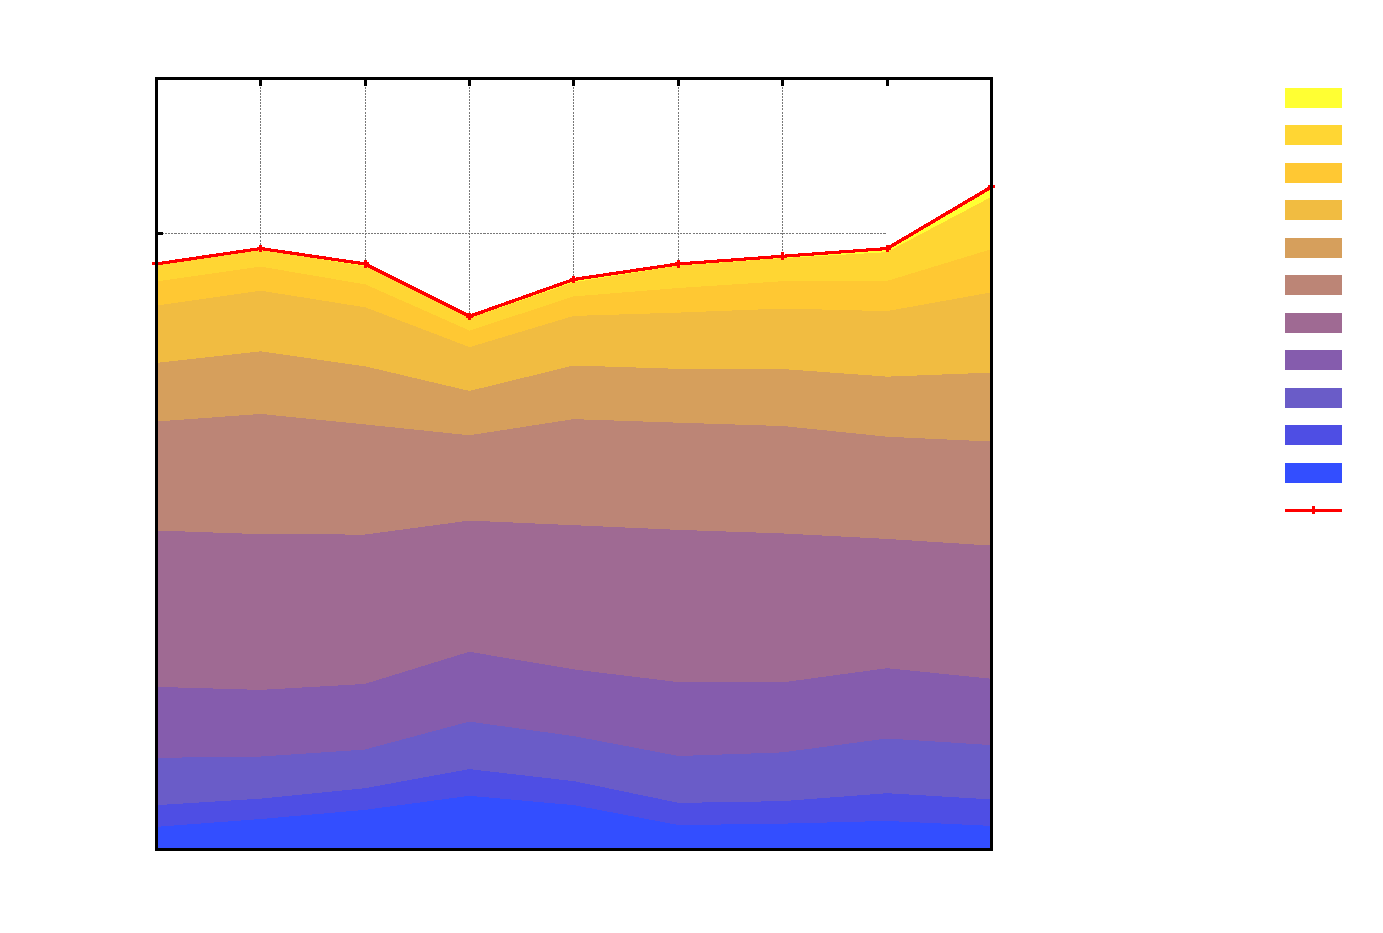
\includegraphics{./plots/house-prices/median-house-prices.eps}}%
    \gplfronttext
  \end{picture}%
\endgroup
